%
% Parameters
%

\ifdefined\fullversion
\else
\def\fullversion{1}    % 0 = conference version; 1 = full version
\fi

\ifdefined\cameraversion
\else
\def\cameraversion{0}    % 0 = long version; 1 = proceedings version
\fi

\def\showoverflow{1}   % 1 = show overflows
\def\allow{1}      % 0 = remove todo command
\def\anonymous{0}      % 1 = anonymous

%
% Document class 
%

\documentclass[envcountsame,runningheads,notitlepage]{llncs}
\ifnum\fullversion=1
\usepackage[a4paper, margin=1.1in]{geometry}
\setlength{\marginparwidth}{2.5cm}
\fi

%
% Custom header
%

\input{tex_files/ZZ_header}

\title{A Survey of SNARKs in Decentralized Finance Systems}
\titlerunning{A Survey of SNARKs in Decentralized Finance Systems}
\date{05/28/2024}

\ifnum\anonymous=0
\author{
  Isaac Thomas\inst{1}
}% Add author name here

\institute{Computer Science \& Engineering, UC San Diego\\
  \href{mailto:isthomas@ucsd.edu}{isthomas@ucsd.edu}
}  % Add institute here

\else
\author{Isaac Thomas} 
\institute{University of California, San Diego}
\fi

\definecolor{darkgrey}{HTML}{272822} 
\definecolor{lightbeige}{HTML}{faf0dd}
\definecolor{hotpink}{RGB}{255, 105, 180} % Hot pink
% \renewcommand{\familydefault}{\sfdefault}

% \pagecolor{lightbeige} 
% \color{lightbeige}

\begin{document}
  \small  
  \maketitle

\begin{abstract}
Succinct non-interactive arguments of knowledge (SNARKs) have seen increasing adoption in decentralized finance (DeFi) systems, where scalability and privacy preservation are of high concern in verifying computation performed on blockchain networks. In particular, SNARKs using pairing-based cryptography are widely used in blockchain infrastructure/applications due to their small proof sizes, fast verification, and easily endowed zero-knowledge properties. In this survey, we review advancements in pairing-based SNARKs relevant to the performance, flexibility and confidentiality of blockchain networks and their hosted applications. Along with fundamental SNARK properties and early work, we discuss alternate characterizations of the complexity class NP, cryptographic primitives, and optimizations modern pairing-based SNARKs collectively employ to verify payments and execution paths through on-chain programs; and we weigh concrete security/performance/privacy tradeoffs emerging from such design choices. Finally, we discuss applications and future SNARK research avenues relevant to verifying on-chain computation.
\end{abstract}

\section{Preliminaries}

\subsection{What is a SNARK?}
\noindent Loosely speaking, a succinct non-interactive argument of knowledge is a short, one-shot proof that one $knows$ some ``witness'' or value $w$ satisfying a claim $C$ related to public input(s) $x$. In practice, $C$ is a claim that $x \in L$, where $L \in \text{NP}$. We give a more formal definition below.\\

\subsubsection{A more formal definition}
\noindent Let the relation $\mathcal{R} = \{(x, w)\} \subseteq \{0, 1\}^{*} \times \{0, 1\}^{*}$ be decidable in deterministic polynomial time, where $|w| = \mathsf{poly}(|x|)\ \forall (x, w) \in \mathcal{R}$. Let $\lambda \in \mathbb{N}$ denote a security parameter. Define the language $L = \{x\ |\ \exists w\ \text{s.t.}\ (x, w) \in \mathcal{R}\}$. A succinct non-interactive argument of knowledge is the tuple of PPT algorithms $(\sf{Setup}, \sf{Prove}, \sf{Verify})$ where:
\begin{itemize}
    \item $\sf{Setup}(1^{\lambda}, \mathcal{R}) \rightarrow \sigma$ receives an input security parameter and relation, and outputs a common reference string (CRS) $\sigma$ containing the ``setup'' terms the prover and verifier will use to construct/verify proofs
    \item $\sf{Prove}(\sigma, x, w) \rightarrow \pi$ receives the CRS, string $x$, and witness $w$ and outputs a proof $\pi$
    \item $\sf{Verify}(\sigma, x, \pi) \rightarrow \{0, 1\}$ receives the CRS, string $x$, and proof $\pi$; it outputs 1 (accepts) or 0 (rejects)
\end{itemize}

\noindent and $\sf{Setup}, \sf{Prove}, \sf{Verify}$ have the following properties:
\begin{itemize}
    \item \textbf{completeness:} If $\pi \leftarrow \sf{Prove}(\sigma, x, w)$ and $(x, w) \in \mathcal{R}$ then $\sf{Verify}$ outputs 1 
    \item \textbf{soundness:} For all possible PPT algorithms $\sf{Prove'}$, if $\pi' \leftarrow \sf{Prove'}(\sigma, x, w)$ and $x \notin L$, then $\sf{Verify}(\sigma, x, \pi') = 1$ with probability at most $\delta_s$ ($\mathcal{V}$ rejects with probability at least $1 - \delta_s$). 
    \item \textbf{knowledge soundness:} For all possible PPT algorithms $\sf{Prove'}$, if $\pi' \leftarrow \sf{Prove'}(\sigma, x)$ and $\sf{Verify}(\sigma, x, \pi') = 1$ with non-negligible probability, then there exists a PPT extractor $\mathcal{E}$ which, given access to the same inputs as $\sf{Prove}$ and $\mathcal{P}$'s random tape, outputs $w$ s.t. $(x, w) \in \mathcal{R}$. 
    \item \textbf{succinctness:} Let $(x, w) \in \mathcal{R}$ and $\pi \leftarrow \sf{Prove}(\sigma, x, w)$. $|\pi|$ is polylogarithmic in $|x|$, prover complexity is quasilinear in $|x|$, and verifier complexity is polylogarithmic in $|x|$. Setup complexity is quasilinear in $|x|$. 
    \item \textbf{non-interactivity:} $\pi$ is generated without any interaction between $\mathcal{P}$ and $\mathcal{V}$ after setup.
\end{itemize}

\noindent As an example, $L$ could be the set of string encodings of satisfiable boolean circuits (there's some input out there making the circuit output `True`. The claim to be proven is that $x \in L$, where $x$ is the encoding of the circuit in question; since $L$ is fixed here, the claim can just be represented by $x$. Our witness $w$ is our potentially secret ``certificate'' proving the validity of the claim.\\

\subsection{Early work}
\noindent Succinct non-interactive arguments of knowledge are preceded by foundational work in complexity theory, probabilistic proofs, and cryptography. First and foremost was the formalization of interactive proofs by Goldwasser et al.\ \cite{ipfirst}, which established a theoretical framework by which a prover $\mathcal{P}$ exchanges a finite number of messages during \textit{interaction} with a verifier $\mathcal{V}$, which issues \textit{random challenges} to $\mathcal{P}$ in order to verify their claim. They also introduced the notion of zero-knowledge.\\ 

\noindent An obvious choice of proof system would involve sending the full ``certificate'' of the given problem's solution to $\mathcal{V}$; however, this is not succinct or zero-knowledge. In light of this, the following question seems natural: do ``short enough'' or \textit{succinct} arguments of knowledge exist for NP? Kilian's construction \cite{kilian} found an affirmative answer to this inquiry (for verification at least) using merkle tree commitments to probabilistically checkable proofs (PCPs), and Micali later showed how to make this argument non-interactive \cite{micalisnark} using the Fiat-Shamir heuristic \cite{fiatshamir}. Despite these breakthroughs, SNARKs constructed from PCPs were undesirable due to massive overhead incurred in proof construction. Many approaches which address this fundamental issue use alternate characterizations of NP -- namely rank-1 constraint systems (R1CS), and algebraic intermediate representations (AIRs) -- which admit means to efficient polynomial identity/property testing. Additionally integrating ``compiled'' interaction and suitable cryptographic commitment schemes can reduce prover complexity, proof length, and verifier complexity.\\

\noindent As seen in Kilian's work, along this path to succinctness lies an interesting and practically necessary avenue: considering only computationally bounded adversaries. In doing so, one can now use cryptographic schemes to encrypt proof elements and verify their integrity. This can enable small proof sizes and fast verification while still making it infeasible to break soundness in polynomial time. Pairing-based cryptography, which allows one to check algebraic relationships between quantities ``in the exponent'' using bilinear functions (behaving like multiplication) on elliptic curve group elements, spurred a sequence of works leading to methods practical enough for real-world blockchain applications. Though faster, all of these methods require stronger assumptions about what information an adversary must know to have produced a particular group element. Due to the use of elliptic curve cryptography (ECC), they also derive their security from the discrete log assumption, which is stronger than the collision resistance assumptions used in other hashing-based methods like STARKs. With the pairing-based denomination of SNARKs and others, the tradeoff between performance and security is a recurring and noteworthy point of comparison.


\subsection{A general ``workflow'' for SNARKs}
Modern SNARKs largely use the "workflow" depicted below to prove/verify computation:
\begin{figure}[htbp]
    \centering
    \begin{tikzpicture}[
        node distance=1.5cm,
        box/.style={rectangle, draw, rounded corners, minimum width=2cm, minimum height=0.8cm, text width=1.9cm, align=center, font=\footnotesize},
        box-highlight/.style={rectangle, draw=red!70, line width=1.2pt, rounded corners, minimum width=2cm, minimum height=0.8cm, text width=1.9cm, align=center, font=\footnotesize},
        arrow/.style={->, >=latex},
        arrow-highlight/.style={->, >=latex, draw=red!70, line width=1.2pt}
    ]
    
    % Define nodes - first row
    \node[box-highlight] (comp) {computation};
    
    % Second row
    \node[box-highlight] (circ) [below left=0.8cm and 0.3cm of comp] {circuit};
    \node[box] (aet) [below right=0.8cm and 0.3cm of comp] {AET};
    
    % Third row
    \node[box-highlight] (r1cs) [below left=0.8cm and 0cm of circ] {R1CS};
    \node[box-highlight] (cust) [below right=0.8cm and 0cm of circ] {custom NP repr.};
    \node[box] (air) [below=0.8cm of aet] {AIR};
    
    % Fourth row
    \node[box-highlight] (polyid) [below right=0.8cm and 0.3cm of r1cs] {poly. EQ};
    \node[box] (cw) [below right=0.8cm and 0.3cm of air] {poly. CW};
    
    % Fifth row
    \node[box-highlight] (crypto) [below=0.8cm of polyid] {pairing-based CC};
    \node[box] (crypto2) [below=0.8cm of cw] {hashing-based CC};
    
    % Sixth row
    \node[box-highlight] (pair) [below=0.8cm of crypto] {PC};
    \node[box] (prox) [below=0.8cm of crypto2] {PPT};
    
    % Define connections - with highlighting for the pairing-based path
    \draw[arrow-highlight] (comp) -- (circ);
    \draw[arrow] (comp) -- (aet);
    
    \draw[arrow-highlight] (circ) -- (r1cs);
    \draw[arrow-highlight] (circ) -- (cust);
    \draw[arrow] (aet) -- (air);
    
    \draw[arrow-highlight] (r1cs) -- (polyid);
    \draw[arrow-highlight] (cust) -- (polyid);
    \draw[arrow] (air) -- (cw);
    \draw[arrow] (cust) -- (cw);
    \draw[arrow] (r1cs) -- (cw);
    
    \draw[arrow-highlight] (polyid) -- (crypto);
    \draw[arrow] (cw) -- (crypto2);
    
    \draw[arrow-highlight] (crypto) -- (pair);
    \draw[arrow] (crypto2) -- (prox);
    
    \end{tikzpicture}
    \caption{A general workflow describing how SNARKs convert computations into verifiable statements. The highlighted path shows the course pairing-based approaches take. Acronyms: AET = algebraic execution trace, AIR = algebraic intermediate representation, CC = cryptographic compilation, CW = codewordx, EQ = polynomial equality, PC = pairing check, PPT = polynomial proximity testing, R1CS = rank-1 constraint system.}
    \label{fig:snark-workflow}
\end{figure}
\noindent Here there are two courses; one reduces to checking polynomial relationships using pairing-based cryptography (left), and the other reduces to checking proximity to a Reed-Solomon code via combination of coding theoretic results and merkle trees. In an interactive setting, the "checks" or "testing" steps might involve randomized interaction with the verifier; but many methods use Fiat-Shamir to have the prover simulate such interaction, which the verifier can check. The result is an interactive protocol compiled into a succinct non-interactive argument of knowledge (the "compilation" here is different from the compilation mentioned in the graph above). To balance coverage, depth, and accessibility, this paper focuses on approaches involving pairing-based cryptography (highlighted paths). We leave the surveying of methods using hashing-based cryptography as future work.

\subsection{Representing the complexity class NP}
\noindent Crucial to modern SNARKs is their representation of NP. How the computation to verify is ``framed'' directly influences how synergistic each method is with algebraic objects like polynomials and the cryptographic methods applied to them. Clearly, one must use an NP-complete language compatible with other aspects of the method in question. The most immediate choice of representation is boolean circuit satisfiability; in light of the use of polynomials, a reasonable sequel is \textit{arithmetic} circuit satisfiability, in which the circuit of importance uses addition gates in place of OR gates, and multiplication gates in place of AND gates. Wires can also take on values in some prime field $F_p$  rather than just 0 or 1. A natural question arises: are there representations of NP that seamlessly connect arithmetic circuit satisfiability with polynomial testing? The answer is yes, and we discuss notable examples of this below.

\subsubsection{Rank 1 Constraint System (R1CS)}
Let $m, n \in \mathbb{N}$, and consider an arithmetic circuit with $m$ gates and $n$ input variables. with A rank-1 constraint system [5] (R1CS) consists of a vector $w \in \mathbb{F}_{p}^{n}$, the matrices $L, R, O \in \mathbb{F}_{p}^{m \times n}$ and the relationship
\begin{align}
Ow = (Lw) \circ (Rw)
\end{align}
A rank-1 constraint system (R1CS) \textit{arithmetizes} the relationships between the left inputs, right inputs, and outputs of each gate, respectively. It assumes that the circuit has been preprocessed so that only multiplication gates remain, with the addition gates instead expressed as sums input to the multiplication gates. Intuitively, row $i$ of $L$ can be seen as a ``selector'' for the values in $w$ that, when linearly combined via row $L_i$, form the left input to gate $i$. The same logic applies for $R$ and $O$. Applying this logic in aggregate yields the above relationship between a Hadamard product of vectors and the desired output vector - in other words, three rank-1 matrices (hence ``rank-1''). This problem is NP-complete with a relatively simple reduction from arithmetic circuit-SAT (follows easily from the loose definition above). One can also view it as a consolidation of the equations in the constraint system used by Bootle et al.[5], which uses two separate equations for multiplication gate constraints and linear constraints.

\subsubsection{Quadratic Arithmetic Program (QAP)}
Connecting the R1CS representation of NP with polynomials involves converting either the rows or the columns of $L, R, O$ into polynomials and creating some relationship that holds if and only if $Ow = (Lw) \circ (Rw)$. Given that for the $i$-th gate we have
\begin{align}
(Oz)_i = \left(\sum_{j=1}^n L_{ij}w_j\right)\left(\sum_{j=1}^n R_{ij}w_j\right)
\end{align}
It could make sense to create a polynomial for each of the $n$ witness variables which evaluate to each $L_{ij}$ given the gate $i$. This would involve interpolating column $j$ of the matrix $L$ into a polynomial $u_j(x)$. The same intuition applies to the matrices $R, O$ (using $v_j(x), w_j(x)$ respectively) and is the idea behind the quadratic arithmetic program (QAP) introduced by Gennaro et al. \cite{snarknopcp}. We focus on the definition of a regular QAP.

\begin{definition}[regular QAP]
A regular Quadratic Arithmetic Program $Q$ over a field $\mathbb{F}_p$ comprises:
\begin{itemize}
    \item The target polynomial $t(x) = \prod_{i=1}^m (x - i)$, where $m$ is the number of gates
    \item Three sets of polynomials $\{u_i(x)\}_{i=0}^n$, $\{v_i(x)\}_{i=0}^n$, and $\{w_i(x)\}_{i=0}^n$, where $u_i(j) = L_{ji}$, $v_i(j) = R_{ji}$, and $w_i(j) = O_{ji}$
\end{itemize}

$Q$ is satisfied by a witness $c \in \mathbb{F}_p^n$ if and only if:
\begin{align}
p(x) = \left(\sum_{i=0}^n c_i u_i(x)\right) \cdot \left(\sum_{i=0}^n c_i v_i(x)\right) - \left(\sum_{i=0}^n c_i w_i(x)\right) = h(x)t(x) \equiv 0 \mod t(x)
\end{align}
\end{definition}

\noindent Here $t(x) | p(x)$ is synonymous with $p(x)$ vanishing at all points which are gate identifiers, which will be true if the gate relationship is indeed satisfied by the given inputs, and will not be true otherwise. QAP satisfiability is also NP-complete with intuitive reductions from arithmetic circuit-SAT and R1CS. Gennaro et al. originally coined QAPs as a way to compute arithmetic circuits, but the relationship to R1CS is more noteworthy given the methods to be discussed, hence the slightly altered presentation.\\

\noindent Though not exhaustive by any means, these two representations of NP yield a connection between the computation being verified, arithmetic circuit satisfiability, and an instance of polynomial divisibility testing. From this point, the polynomial divisibility check can be verified in a hidden fashion using pairing-based cryptography. This idea is used by virtually all pairing-based methods, with modifications to the constraint system and the polynomial relationship being checked.

\subsection{Polynomial Properties}
\noindent As mentioned, modern SNARKs reduce proving/verifying statements about computation to polynomial identity/property testing via suitable characterizations of NP. A natural question about this arises: why polynomials over other mathematical objects? The answer lies in how little information one needs to distinguish between two arbitrary polynomials, which is a consequence of the following lemma.

\subsubsection{Schwarz-Zippel lemma}
\noindent Let $f(x_1, x_2, \dots x_n) \in R[x_1 \dots x_n]$ be a nonzero polynomial in $n$ variables defined over an integral domain $\mathbb{F}^{n}$. Suppose the element $(a_1, a_2, \dots a_n)$ is selected uniformly at random from a finite subset $S \subset \mathbb{F}^n$. Then 
$\Pr(f(a_1, a_2, \dots a_n) = 0) \le \frac{\text{deg}(f)}{|S|}$
where $\text{deg}(f)$ is the maximum sum of the degrees of any term's variables. It immediately follows that if $f = g-h$, as $g$ and $h$ are distinct since $f$ is not zero; then for a randomly sampled point $(a_1, \dots a_n)$, the probability that 
$(g-h)(a_1, \dots a_n) = 0 \Leftrightarrow g(a_1, \dots a_n) = h(a_1, \dots a_n)$
is identically bounded. In other words, $g$ and $h$ will output different values at $(a_1 \dots a_n)$ with high probability if they are not equal, assuming the $d$ and $\mathbb{F}$ are chosen appropriately $d \ll |F|$. Thus, given the right choice of degree and field size, a verifier will still be able to distinguish between two unequal polynomials with high probability using a single evaluation point.\\ 

\noindent Schemes relying on this property would yield shorter proofs, since we need a single evaluation point; faster prover complexity, since polynomial evaluation has many known efficient algorithms over both finite fields and the real numbers; and faster verification, since checking a polynomial identity can be done quickly via point evaluation without significant soundness loss. Thus, if a succinct argument system can verify identities resemblent to this one, it would warrant the characterization of the claim being proven in a manner easily convertible to a collection/combination of polynomials.

\subsection{Pairing-Friendly Elliptic Curve Cryptography}

\noindent Pairing-based cryptography, which allows one to check algebraic relationships between quantities ``in the exponent'' using bilinear functions on arbitrary source group elements (usually from elliptic curve groups), is a heavily used cryptographic primitive in modern SNARKs. Elliptic curve groups are preferred here due to small key sizes -- determined by the size of the base field the coordinates of the points from. There is also a natural group operation over elliptic curve points behaving like addition; when compounded with the hardness of computing discrete logarithms over elliptic curve groups, this yields a scheme for additively homomorphic encryption. Pairings can render this scheme \textit{doubly} homomorphic due to the properties of bilinear pairings. This paper abstracts the details of elliptic curve groups for brevity; we instead focus on the properties they exhibit which make them a useful component of pairing-based cryptography.\\

\noindent More formally, suppose we have two cyclic elliptic curve groups $\mathbb{G}_1$ and $\mathbb{G}_2$ generated by elements $G_1$ and $G_2$, respectively. We denote the scalar multiple of a point $P \in \mathbb{G_1}$ by $kP$, which is just the same as $k$ additions of $P$ and $k \in \mathbb{F}_s$ where $\mathbb{F}_s$ is some scalar field. For a bilinear pairing $e: \mathbb{G}_1 \times \mathbb{G}_2 \to \mathbb{G}_t$ where $P_1 \in \mathbb{G}_1$ and $P_2 \in \mathbb{G}_2$, we have the following properties:
\begin{itemize}
    \item for $s \in \mathbb{F}$, $e(P_1, sP_2) = e(sP_1, P_2) = e(P_1, P_2)^s$
    \item for $Q_1 \in \mathbb{G}_1$, $e(P_1+Q_1, P_2) = e(P_1, P_2) e(Q_1, P_2)$
    \item for $Q_2 \in \mathbb{G}_2$, $e(P_1, P_2+Q_2) = e(P_1, P_2) e(P_1, Q_2)$
    \item $e(G_1, G_2)$ generates $\mathbb{G}_t$ (non-degeneracy)
\end{itemize}

These properties make it easy to check multiplicative relationships. For instance, suppose we have three polynomials $A(x), B(x), C(x)$ and we want to check that $A(\alpha)B(\alpha) = C(\alpha)$ for some input $\alpha$. From bilinearity of $e$ It follows that 
\begin{align}
e(G_1, G_2)^{A(\alpha)B(\alpha)} &= e(G_1, G_2)^{C(\alpha)} \\
\Leftrightarrow e([A(\alpha)]_1, [B(\alpha)]_2) &= e([C(\alpha)]_1, G_2)
\end{align}
where $[A(\alpha)]_1 = A(\alpha)G_1$ (same idea for the other values). So if we can reduce checking circuit satisfiability to checking a polynomial relationship, we can send elliptic curve points as proof elements with which the verifier would perform such a pairing check. The complexity of a naive pairing computation is quasi-quadratic in the target group size, but there are pairing-friendly choices of elliptic curve groups which make this operation faster. Most importantly, the number of pairings to be performed does not depend on the size of the computation being verified.

\subsection{Polynomial commitment scheme (PCS)}

\noindent A polynomial commitment scheme is a protocol by which a prover claims they know a polynomial $f(x)$ satisfying some relationship, and a verifier checks this claim. A noteworthy example of such a relationship is that $f(y) = z$ for some fixed $y, z$. We detail a noteworthy polynomial commitment scheme for this exact task known as the KZG commitment scheme, named after the authors Kate et al. Kate-Zaverucha-Goldberg (KZG) commitments facilitate verification of the commitment made by a prover $P$ to a specific polynomial $f$ meeting certain requirements [7]. Suppose $P$ wants to prove they know $f$ of degree $d$ such that $f(\beta) = z$. It follows that $f(X) - z$ is divisible by $(X - \beta)$, so we should be able to construct
\begin{align}
h(X) = \frac{f(X) - z}{X - \beta}
\end{align}
since we know $f$. $P$ commits to $f$ and $h$ by their hidden evaluations on some $\alpha$ agreed upon in advance by the $P$ and the verifier $V$. In practice, the evaluations are hidden via scalar multiplication by an elliptic curve group generator $g_1 \in \mathbb{G}_1$. This scheme uses two elliptic curve groups for this purpose, so assume the point $g_2$ generates the EC group $\mathbb{G}_2$. Let $[a]_i = ag_i \in \mathbb{G}_i$. Suppose $\mathcal{P}$ and $\mathcal{V}$ agree on a \textit{trusted setup} containing the hidden terms 
\begin{align}
\{[1]_1, [\alpha]_1, [\alpha^2]_1, \dots [\alpha^{d}]_1, [1]_2, [\alpha]_2\}
\end{align}

$P$ sends $[f(\alpha)]_1$ and $[h(\alpha)]_2$. $V$ then sends a challenge point $\gamma$ to which $\mathcal{P}$ responds with $[f(\gamma)]_1$ and $[h(\gamma)]_1$. $V$ then checks that $f(\gamma) - z = h(\gamma)(\gamma - \alpha)$ where $h$ was constructed from the evaluation requirement we wanted to prove that $f$ satisfies. For a bilinear pairing function $e : \mathbb{G}_1 \times \mathbb{G}_2 \to \mathbb{G}_t$, $\mathcal{V}$ checks that 
\begin{align}
&e([f(\gamma) - z]_1, g_2) = e([h(\gamma)]_1, [\gamma]_2 - [\alpha]_2) \\
&\Leftrightarrow e(g_1, g_2)^{f(\gamma) - z} = e(g_1, g_2)^{h(\gamma)(\gamma - \alpha)} \\
&\Leftrightarrow  f(\gamma) - z = h(\gamma)(\gamma - \alpha)
\end{align}

\noindent KZG commitment schemes require constant size communication since the polynomials involved can be collapsed to a point without losing virtually any distinguishability. Given their use of elliptic curve points to meet this end, their security depends on the hardness of computing elliptic curve discrete logarithms (find $\alpha$ given the points $g$ and $\alpha g$), for which no classical polynomial time algorithm is known \cite{ecdlp}. The drawbacks of using this scheme include the need to generate a trusted setup upstream, and the reliance on the discrete log assumption (not post-quantum).\\

\noindent There are other general and protocol-specific commitment schemes which check slightly different polynomial relationships than KZG or avoid pairing-based cryptography entirely. But we opt for this example to give an idea of commitment schemes making use of pairings, as this is relevant to every modern pairing-based SNARK discussed.

\subsection{Turning interactive protocols non-interactive}
\noindent nothing.

\section{Circuit-specific pairing-based SNARKs}
\noindent The seminal PCP theorem yielded a powerful characterization of NP as the set of languages with polynomial-time PCP verifiers. However, early work on pairing-based SNARKs was actually motivated by the possibility of succinct arguments of knowledge using a representation \textit{more suitable than PCPs} for integration with cryptographic primitives. Several other works came close to meeting this end but could not attain sublinear proof size.\\

\noindent To this end, Gennaro et al. \cite{snarknopcp} coined quadratic span programs (QSP) and quadratic arithmetic programs (QAP) as a way of representing boolean/arithmetic circuit-SAT with polynomials, along with succinct NIZK for both QSP-SAT and QAP-SAT. Although the QSP construction is noteworthy, we limit discussion to their QAP-related construction due to the easier connection to arithmetic circuits and polynomials. We recall the strong QAP form here:
\begin{align}
\underbrace{\left(\sum_{j=1}^n a_i v_i(x)\right)}_{\text{left inputs}} \cdot \underbrace{\left(\sum_{j=1}^n b_i w_i(x)\right)}_{\text{right inputs}} - \underbrace{\left(\sum_{j=1}^n c_i y_i(x)\right)}_{\text{outputs}} = h(x) t(x) \equiv 0 \mod t(x)
\end{align}

\noindent The idea was to leverage the notion of some additively homomorphic encoding $E$ -- namely, an injective, additively homomorphic function for which inversion is difficult -- to compile a QSP/QAP instance into a proof containing just 9 group elements (non-ZK). We detail the non-zero-knowledge version here for clarity. Denote $E(x)$ by $[x]$. The prover $\mathcal{P}$ solves for $h(x)$ and sends

\begin{align}
    \pi = \Big(&[v_{mid}(s)], [w(s)], [y(s)], [h(s)], \\ 
    &[\alpha v_{mid}(s)], [\alpha w(s)], [\alpha y(s)], [\alpha h(s)], \\ 
    &[\beta_v v_{mid}(s) + \beta_w w(s) + \beta_y y(s)]\Big)
\end{align}

where $\alpha, s, \beta_v, \beta_w, \beta_y \in \mathbb{F}_p, $ are secret random preprocessing elements; $v_{mid}(s), w(s), y(s)$ are the witness-weighted combinations of the wiring polynomials in the QAP; and $h(s)$ is the evaluation of the quotient polynomial an honest prover would know. In particular, $v_{mid}(x) = \sum_{k \in \mathcal{I}_{mid}} a_k v_k(x)$ where $\mathcal{I}_{mid}$ are the indices corresponding to private circuit inputs. The verifier in turn checks 5 equations using the additive properties of $E$. In particular, the verifier receives the following proof $\pi'$ \textit{which it does not yet know is valid}, hence the new notation of elements reminiscent of those in $\pi$:
\begin{align}
\pi' = (\pi_{v_{mid}}, \pi_{w}, \pi_{y}, \pi_{h}, \pi_{v'_{mid}}, \pi_{w'}, \pi_{y'}, \pi_{h'}, \pi_{z'})
\end{align}

and checks 6 equations; the first one checks the QAP relation, and the rest essentially compare proof elements with themselves, but recomposed in a way that tests if the prover knows the unhidden QAP elements:
\begin{align}
(v_0(s) + v_{in}(s) + \pi_{v_{mid}})(w_0(s) + \pi_w) - (y_o + \pi_{y}) - \pi_h t(s) &= 0 \\
\alpha v_{mid}(s) - v'_{mid}(s) &= 0 \\
\alpha w(s) - w'(s) &= 0 \\
\alpha y(s) - y'(s) &= 0 \\
\alpha h(s) - h'(s) &= 0 \\
z'(s) - \gamma \beta_v v_{mid}(s) - \gamma \beta_w w(s) - \gamma \beta_y y(s) &= 0
\end{align}
where $v'_{mid}(s)$ is encoded in $\pi_{v'_{mid}}$, $w'(s)$ is encoded in $\pi_{w'}$, and so on. This is done ``in the exponent'' using pairings, but we provide the unhidden equations for clarity.\\

\noindent GGPR uses a \textit{strong} QAP for their scheme, which uses a different set of coefficients for each sum in the QAP equation. This mandates a \textit{strengthening step} in which extra constraints between the coefficient sets are materialized, tripling prover work and preprocessing size. Parno et al. \cite{pinocchio} made the simple optimization of using a \textit{regular} QAP, which uses the same set of coefficients for each sum in the QAP expression. We recall the regular QAP form:
\begin{align}
\underbrace{\left(\sum_{j=1}^n a_i v_i(x)\right)}_{\text{left inputs}} \cdot \underbrace{\left(\sum_{j=1}^n a_i w_i(x)\right)}_{\text{right inputs}} - \underbrace{\left(\sum_{j=1}^n a_i y_i(x)\right)}_{\text{outputs}} = h(x) t(x) \equiv 0 \mod t(x)
\end{align}
\noindent The use of the same $a_i$ across all sums eliminated the need for the strengthening step without any noteworthy compromises, although it required modifications to proof elements and verification checks that ensure consistent use of coefficients in QAP terms. The resulting proof sent by the prover looks slightly different. Consider the following preprocessing elements (among others):
\begin{align}
r_v, r_w, s, \alpha_v, \alpha_w, \alpha_y, \beta, \gamma &\overset{R}\leftarrow \mathbb{F} \\
r_y &= r_v r_w \\
g_v &= r_v G \\
g_w &= r_w G \\
g_y &= r_y G
\end{align}

\noindent The prover $\mathcal{P}$ would send 
\begin{align}
    \pi_2 = \Big(&[v_{mid}(s)], [w_{mid}(s)], [y_{mid}(s)], [h(s)], \\
    [&\alpha_v v_{mid}(s)], [\alpha_w w_{mid}(s)], [\alpha_y y_{mid}(s)], \\
    [&\beta_v v_{mid}(s) + \beta_w w_{mid}(s) + \beta_y y_{mid}(s)]\Big)
\end{align}

\noindent where like before, $v_{mid}(x) = \sum_{k \in \mathcal{I}_{mid}} a_k v_k(x)$ and likewise for $w_{mid}(x)$, $y_{mid}(x)$. Similar to GGPR, the verifier receives
$$
\textbf{THE POTENTIALLY VALID PROOF THE VERIIFER RECEIVES}
$$
and checks the following pairing-based equations:
\begin{align}
e([v_0(s) + v_{in}(s) + v_{mid}(s)]_1 \cdot [w_0(s) + w_{in}(s) + w_{mid}(s)]_1, G_2) = \\
([t(s)]_1, [h(s)]_2) \cdot e([y_0(s) + y_{in}(s) + y_{mid}(s)]_1, G_2) \\
e([r_v v'_{mid}(s)], G) = e([v_{mid}(s)], [r_v \alpha]) \\
e([r_w w'_{mid}(s)], G) = e([w_{mid}(s)], [r_w \alpha]) \\
e([r_y y'_{mid}(s)], G) = e([y_{mid}(s)], [r_y \alpha]) \\
e(z'(s), [\gamma]) = e([r_v v_{mid}(s) + r_w w_{mid}(s) + r_y y_{mid}(s)], [\beta \gamma])
\end{align}

\noindent Imaginably, this form of QAP became a precedent for later work. In particular, Groth used regular QAPs and stronger knowledge assumptions to produce a SNARK with proofs containing just three elliptic curve group elements while preserving succinct verification. The improvements here were largely due to more aggressive compilation of QAP polynomial elements into single setup terms, which decreased setup size and proof size at the expense of needing stronger assumptions about what witness information the prover knows.\\

\noindent While some would regard them as extreme, these stronger knowledge assumptions are not necessarily uncalled for; SNARKs for NP cannot exist without non-falsifiable assumptions to begin with, and reduction in proof length could also be regarded as "worth it" on this front. Consequently, Groth's work (colloquially known as groth16) saw large adoption in blockchain systems verifying homogeneous computation; applications like Tornado Cash and Railgun use this method to verify withdrawals from privacy-preserving pools, for instance.

\section{Circuit-independent (universal) pairing-based SNARKs}
\noindent Homogeneous computation aside, circuit-specific pairing-based methods have a couple of noteworthy shortcomings. The first of these as noted by Groth \cite{grothupdatable} is that there is no way of ensuring the deployers of the SNARK in question have disposed of the secret randomness used to generate the trusted setup. The second and more important issue is a lack of flexibility due to the use of computation-dependent (non-universal) preprocessing. As an example, we depict the groth16 trusted setup here. As in the QAP definition, the $u_i(x), v_i(x), w_i(x)$ encode the contribution of the $i$-th witness component to left input, right input, and output of gate $x$ respectively. 
\begin{align}
\sigma = \Big( 
    &[\alpha]_1, [\beta]_1, [\gamma]_1, [\delta]_1, \{[x^i]_1\}_{i \in [0, n-1]}, \{[\gamma^{-1}(\beta u_i(x) + \alpha v_i(x) + w_i(x))]_1\}_{i \in [0, \ell]}, \\
    &\{[\delta^{-1}(\beta u_i(x) + \alpha v_i(x) + w_i(x))]_1\}_{i \in [\ell+1, m]}, \\
    &\{[\delta^{-1} x^i t(x)]_1\}_{i \in [0, \deg(h)]}, [\beta]_2, [\gamma]_2, [\delta]_2, \{[x^i]_2\}_{i \in [0, n-1]}
\Big)
\end{align}

\noindent As is the case with other discussed methods, the contributions of the $i$-th witness component to gate $x$ are ``stuck'' in the encrypted $u_i(x), v_i(x), w_i(x)$ (not the component's value, but its index). Thus if the circuit wiring changes, these polynomials must change to reflect this. Updating the setup incrementally, however, is not possible for two reasons, either of which is sufficiently limiting. The first is the hidden $u_i(x), v_i(x), w_i(x)$ are interpolated from relationships between witness components and the gates they feed into. Adding a new gate and its associated wire connections would require adding a new data point to each of these polynomials. Thus, one would have to re-interpolate all of them which is not possible without violating cryptographic assumptions (since they are encrypted) or regenerating the entire setup, which defeats the purpose of updates. Another related reason concerns the setup's combination of these hidden polynomial terms, such as the $[\beta u_i(x) + \alpha v_i(x) + w_i(x)]_1$. Groth \cite{grothupdatable} showed these setup terms could be used to extract the the constituent monomials and ultimately break soundness if the setup allowed updates. These observations suggest that the conception of a QAP-based updatable SNARK is unlikely, and that different approaches are necessary. Such approaches should be \textit{universal}, in the sense that they allow proving computation of any structure up to a certain size; and \textit{updatable}, meaning that the trusted setup can be efficiently updated by any party and remains sound if at least one setup contributor is honest. This idea becomes highly relevant when deploying blockchain systems using SNARKs with trusted setups. After one update to the setup (which can be performed by anyone with a corresponding proof), users do not have to worry about the network being subverted by its deployers or other adversaries. As they stray from the QAP-based paradigm which seems to be ``maxed out'', the following methods use a more diverse set of arithmetizations and polynomial checking to fulfill these universality/updatability related goals; consequently, these are where most of the notable points of comparison arise. For this reason, our discussion of security is significantly more sparse in the following sections; that said, the most noteworthy methods prove security in the algebraic group model (AGM) \cite{agm}, in which adversarial algorithms can exploit group-specific structure (weaker security assumptions than than GGM). \\

\noindent To meet universality/updatability-related ends, Groth \cite{grothupdatable} produced a universal and updatable scheme using a multivariate polynomial encoding of QAP elements. Although this scheme had constantn proof size, constant verification complexity, and a linear-time procedure by which a linear-size circuit-specific setup could be produced as needed, true universality required quadratically many terms w.r.t circuit size. Furthermore, SRS updates would take a quadratic number of group exponentiations and update verification a linear number of pairing operations. For circuits with millions of gates this is impractical. However, this attempt hints that a SNARK with linear-size universal \& efficiently updatable setup could be attainable if the setup terms are univariate (and monomial). Maller et al. achieved this with Sonic, which draws inspiration from techniques of Bootle et al. \cite{bootlezkargs} reducing circuit satisfiability to checking Laurent polynomials encoding a Hadamard matrix product (models mul. gate operations) paired with a linear constraint system (models wire connections \& addition gates). They also use a permutation argument inspired by Bootle et al. \cite{grothshuffle} to enforce correct copying of values across linked wires. The setup contains only univariate monomials and therefore requires linear space, though it is twice the space one would like due to the presence of $X^{-i}$ term for every $X^i$ term (loosely written). Being composed of monomials, the setup can be updated by any party supplying a corresponding proof of update validity. In a realistic deployment of this scheme, the setup would not be circuit dependent, and a single update could eliminate the risk that the deployers still hold valid setup secrets.\\ 

\noindent Though significant in its own right, Sonic suffers from two shortcomings. First, it is not fully verifier-succinct. Second and foremost, there are large constants in the proof construction complexity. A likely cause is the attempt to accommodate for $n$-fan-in circuits whose gates can accept arbitrarily many inputs. While a reasonable generalization, this allows any given linear constraint the ability to use arbitrarily many witness inputs, requiring the use of entire witness and selector vectors for each constraint. It also causes a bloated permutation argument since a given gate may require arbitrarily many copy constraints between its own inputs and outputs from preceding gates that feed into it. Gabizon et al. \cite{plonk} addressed these issues with a simplifying assumption that may not catch one's eye, but turns out to have important performance implications: simply let each circuit gate take two inputs. The impact of this is twofold. Firstly, it enables a much simpler constraint representation of arithmetic circuit-SAT, where for an $n$ gate circuit we have the following constraint for gate $i$. Here $a_i, b_i, c_i$ the indices in $\mathbf{x}$ corresponding to the left input, right input, and output of the $i$-th gate, respectively; and $\mathbf{q_L}, \mathbf{q_R},\mathbf{q_O},\mathbf{q_M},\mathbf{q_C},$ are ``selector vectors'' determining which gate-related values partake in the constraint. This allows one to express addition or multiplication gates in the same constraint by setting $(\mathbf{q_L})_i, (\mathbf{q_R})_i, (\mathbf{q_M})_i$ accordingly. 
\begin{align}
(\mathbf{q_L})_i \cdot \mathbf{x}_{(\mathbf{a})_i} + (\mathbf{q_R})_i \cdot \mathbf{x}_{(\mathbf{b})_i} + (\mathbf{q_O})_i \cdot \mathbf{x}_{(\mathbf{c})_i} + (\mathbf{q_M})_i \cdot (\mathbf{x}_{(\mathbf{a})_i} \cdot \mathbf{x}_{(\mathbf{b})_i}) + (\mathbf{q_C})_i = 0
\end{align}

    % &\Leftrightarrow \textbf{q}_{a} \circ \textbf{a} + \textbf{q}_{b} \circ \textbf{b} + \textbf{q}_{M} \circ (\textbf{a} \circ \textbf{b}) + \textbf{q}_{C} \circ \textbf{c} = \textbf{0}

\noindent During proof construction, these terms are collected into polynomials $q_L(x), a(x), q_R(x), b(X),$ etc. and combined in the same manner as the original constraint equation. Secondly, the 2-fan-in assumption enables optimizations to the permutation argument inspired by Groth et al. and Maller et al. \cite{grothshuffle, sonic}. While sonic used a product check accounting for the arbitrarily many copy constraints per gate, each product check per gate involves three terms in the numerator and denominator each, resulting in a ``grand product'' used in proof construction. We show the non-zero-knowledge version here, but adding ZK properties requires shifting this equation by adding a ``masking'' polynomial that still vanishes on the desired domain in order to not corrupt the expression.
\begin{align}
    z(X) &= L_1(X) + \\
    &\sum_{i=1}^{n-1} L_{i+1}(X) \prod_{j=1}^{i} \frac{(w_j + \beta\omega^j + \gamma)(w_{n+j} + \beta k_1\omega^j + \gamma)(w_{2n+j} + \beta k_2\omega^j + \gamma)}{(w_j + \beta\sigma^*(j) + \gamma)(w_{n+j} + \beta\sigma^*(n+j) + \gamma)(w_{2n+j} + \beta\sigma^*(2n+j) + \gamma)}
\end{align}

\noindent where $L_i(x) = \frac{X^n - 1}{X - \omega^i}$ is the $i$-th Lagrange basis polynomial defined over the $n$-th roots of unity (gives 1 when $X = \omega^i$ and 0 otherwise). Notably, the polynomial check works well with a common optimization to PlonK's invocation of KZG scheme; by representing the hidden monomials in the Lagrange basis, the point evaluations of polynomials can be computed in $O(d)$ operations where $d$ is the degree of the polynomial in question, which is faster than the $O(d \log d)$ complexity for interpolation via inverse FFT \& subsequent evaluation. The pairing check performed by the verifiere is also ``fixed argument'' in the second source group, enabling both of only 2 pairings the verifier performs to be 30\% faster than the traditional pairing \cite{fapairings}.\\

\noindent The combination of flexibility, intuitive arithmetization, and better efficiency has made PlonK a gateway to other methods increasing expressiveness and performance, with important implications for so-called ``zero-knowledge virtual machines'' (zkVMs). Ambrona et al. \cite{turboplonk} proposed methods to optimize the constraint system used, as well as optimized circuits for PlonK-based verifiable implementations of the ``SNARK-friendly'' Poseidon hash function \cite{poseidon}. For zkVM operations less compatible with SNARK systems, Gabizon et al. proposed Plookup \cite{plookup} which adapts the PlonK permutation argument to verify that a set of values is present in some predetermined table; this is particularly useful for constraining the correctness of zkVM operations involving nonlinear operations that would make the resulting circuits / constraint system inefficient to verify. A notable example is a ``SNARK-unfriendly'' hash function like SHA-3 \cite{sha3}, which has many nonlinear bit-mixing operations. Variations like halo2 \cite{halo2} and plonky2 \cite{plonky2} combine the PlonK arithmetization with commitment schemes inspired by Bulletproofs \cite{bulletproofs} and FRI \cite{fri} respectively to shed the need for a trusted setup at the expense of slower verification. These two advancements highlight the customizability of the PlonK system, which is futher explored among other methods in the following sections.

% Chiesa et al. improved upon this with Marlin \cite{marlin}, a more verifier-succinct approach which cryptographically compiles a ``sparsity-friendly'' polynomial representation of an R1CS instance for the verifier to check algebraic consistency of via pairings. Within, both methods make use of bi-variate and univariate KZG commitments, respectively; more importantly, they also make use of \textit{permutation arguments}, which prove the correct copying of values in consecutive circuit wires. As a key occurrence of flexibility-performance tradeoff, the latter sub-argument is necessary due to the encoding of witness-gate relationshiphs directly in the proof instead of the setup.\\

\section{Applications}

\subsection{Privacy-preserving pools}
\noindent Traditional blockchain network innerworkings expose transaction details, making privacy preservation nontrivial at the application layer. Fortunately, modern SNARKs can help address this issue when endowed with zero-knowledge properties. Applications like Tornado Cash \cite{tornadocash} allow one to deposit funds from wallet $A$, then withdraw the funds to a different wallet $B$ without revealing the link between the two addresses on-chain. The user has to prove that they are the owner of the depositing wallet using a groth16 proof of deposit note membership in a Merkle tree maintained by the Tornado Cash smart contracts on-chain. The homogeneous omputation structure and need for succinct proofs/verification due to tight EVM smart contract gas limits make groth16 a suitable choice.  
\begin{figure}[t]
\centering
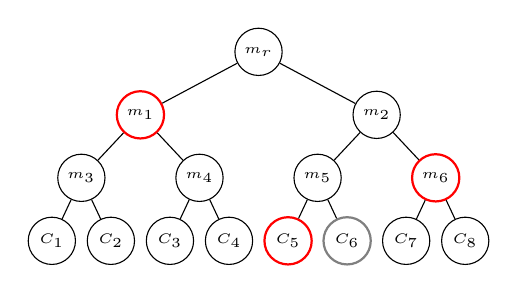
\begin{tikzpicture}[
    level 1/.style={sibling distance=30mm, level distance=8mm},
    level 2/.style={sibling distance=15mm, level distance=8mm},
    level 3/.style={sibling distance=7.5mm, level distance=8mm},
    every node/.style={draw, circle, minimum size=6mm, inner sep=0pt, font=\tiny}
]
    % Root node
    \node {$m_r$}
        % Level 1
        child {node[draw=red, line width=0.8pt] {$m_1$}
            % Level 2
            child {node {$m_3$}
                % Level 3
                child {node {$C_1$}}
                child {node {$C_2$}}
            }
            child {node {$m_4$}
                % Level 3
                child {node {$C_3$}}
                child {node {$C_4$}}
            }
        }
        child {node {$m_2$}
            % Level 2
            child {node {$m_5$}
                % Level 3
                child {node[draw=red, line width=0.8pt] {$C_5$}}
                child {node[draw=gray, line width=0.8pt] {$C_6$}}
            }
            child {node[draw=red, line width=0.8pt] {$m_6$}
                % Level 3
                child {node {$C_7$}}
                child {node {$C_8$}}
            }
        };
\end{tikzpicture}
\caption{Merkle tree with authentication path (in red) for commitment $C_6$ (in gray)}
\label{fig:merkle-tree}
\end{figure}

\subsection{Privacy-preserving blockchains}
\noindent Beneath the application layer there are blockchains utilizing zero-knowledge properties of SNARKs for infrastructural privacy preservation. For each transaction submitted, such systems must obscure the source, relevant currencies, amounts used, and payment recipients. Zerocash \cite{zcash} is a notable example of a network that does such a thing. Intended to be a privacy-preserving version of Bitcoin \cite{bitcoin}, Somewhat similar to (and preceding) Tornado Cash, Zerocash the unspent-transaction-output (UTXO) model, where transactions create so-called ``unspent funds'' that the party who ``owns'' them is entitled to spend. When they do spend those funds, another record of ``unspent funds'' for the recipient of the spending is created. These UTXO records are stored in a merkle tree, and spending funds requires proving knowledge of a leaf in the tree corresponding to the funds. Early versions of Zerocash used groth16 for this, but the NU5 upgrade of 2022 switched to the universal halo2 proof system \cite{halo2}, which enables a combination of a PlonK-style arithmetization and Bulletproofs-style commitment scheme \cite{bulletproofs} requiring no trusted setup at the expense of verifier performance.

\subsection{Verifiable Virtual Machines (VVM)}
\noindent Multiple ``Zero-knowledge virtual machines'' (zkVMs) \cite{scrollzkevm, polygonzkevm, sp1, risc0, openvm} have emerged as architecture-specific and general solutions for proving validity of layer-2 transaction batches on the layer 1 (L1) chains settling them. We use the more accurate phrase ``verifiable virtual machine'' (VVM) since succinctness is a higher priority than zero-knowledge in most L2 architectures. Sitting at the execution layer of the blockchain node implementation, the VVM is responsible for executing calls to smart contracts, generating corresponding execution traces/witnesses, and generating proofs of correct execution for each batch of transactions. PlonK-style variants have been a popular first approach due to the diverse computation structure and lookup-style arguments for verifying ``SNARK-unfriendly'' operations. Many VVM implementations use circuit domain-specific languages (DSLs) like halo2 to implement the circuits constraining the computation details. \\

% \noindent A crucial point of consideration here is that not all computations performed in VVMs are ``SNARK-friendly''; a prime example of this is hash functions like SHA256 which use non-linear or non-algebraic operations like bit mixing. This can cause the circuits constraining this computation to be overly complex and inefficient. To meet this end, lookup-based methods are of great interest here since they can avoid constraining ``SNARK-unfriendly'' operations directly without losing soundness. An example of this is lies in the proof for validity of transaction that called a contract function using \texttt{sha256()}. Instead of constraining the exact sha-256 computation, the prover and verifier would agree on a publicly known table of acceptable inputs and outputs for SHA-256, which the prover commits to as part of the proof. The verifier does not need to know the whole table - they just need to know a commitment to the one considered correct. This can then be compared with what the prover committed to.\\

\section{Future Research}

\subsection{Post-quantum algebraically-friendly SNARKs}
\noindent Though multiple of the SNARKs discussed are practical from a performance standpoint, quantum computers may render them useless from a security standpoint in the near future. As a result, there is a strong effort to develop efficient enough post-quantum SNARKs. To this end, many works \cite{starks, ligero, fractal, spartan, jolt} use hashing-based Reed-Solomon proximity testing methods \cite{fri}, which relies on the hardness of computing hash function collisions. While such approaches are believed to be post-quantum secure, the cryptographic primitives used offer no additively homomorphic structure enabling the recursive composition of smaller proof elements \& faster verification we see in pairing-based methods. Albrecht et al. \cite{lattice1} made some progress in this direction via a lattice-based SNARK with logarithmic-time verification; it derives security from the hardness of the short integer solution (SIS) problem in lattices. Future work that decreases prover/verifier complexity could realize practical SNARKs using additively homomorphic post-quantum encryption, which virtually every blockchain would need in a post-quantum era.

\subsection{Automated verification of SNARK methods/applications}
\noindent Layer 2 blockchains collectively hold tens of billions of dollars \cite{l2beat} protected by the integrity of SNARK methods used to verify block validity; if the methods/implementations have soundness bugs, an adversary could prove an invalid state transition for financial gain and steal funds. There are two promising avenues to mitigate this risk. The first is formal verification of SNARKs in mechanized cryptographic models using Lean 4 and other methods \cite{arklib, lean4, joltfv}. Though very promising and easily updatable, there are still many gaps to fill. Furthermore, the periodic introduction of new methods will require constant updates to the relevant types and theorems. Nonetheless, seeking formal guarantees on SNARK behavior could eliminate entire classes of soundness bugs in L2-related implementations, lowering risks of fund theft. The second and more targeted direction concerns automated detection of nondeterministic circuit behavior using symbolic execution and SMT solvers. An example of this is Picus \cite{picus}, which has been used to verify parts of the Risc Zero VM \cite{risc0}. Preliminary work by Chaliasos et al. \cite{sok} has found that circuit-related soundness bugs are the most frequent kind of bug by a huge margin, suggesting that building upon this existing work will be important especially as zkVM implementations become more complex. LogUp-based arguments \cite{logup} for zkVMs like SP1 \cite{sp1} based on interacting sub-witnesses would be a necessary target of future work in this domain.

% \subsection{Integration of optimizations to pairing-based cryptography}
% \noindent optimize miller function\\
%
% \subsection{Standardized benchmarks for pairing-based methods (and others)}
% \noindent Current SNARK benchmarks lack standardization by the computation being verified.\\


% \subsection{Proof aggregation \& Distributed Proving}
% \noindent As one would expect, proof generation remains the performance bottleneck in most SNARKs (pairing-based or not). In a world where computational resources are quite asymmetrically distributed (DeFi being no exception), it would be sensible to be able to outsource more intensive computations within the same proof to another party; naturally they would include a proof that such computation was done correctly. \textbf{Is there any work on this right now}. A similar idea emerges when we consider distributed proving of a statement by segmenting the \textit{statement} instead of the \textit{proof components}. Each delegated prover would then have to prove that a given subcircuit has an assignment which produces some desired value, then all of these proofs would get aggregated along with a proof that the aggregation was performed correctly.\\
%
%
% \subsection{Extending pairings to higher-degree operations}
% \noindent nothing\\


\newpage
\ifnum\fullversion=0
  \bibliographystyle{splncs03}
 \else
   \bibliographystyle{alpha-short}
 \fi
\bibliography{cryptobib/abbrev3,cryptobib/crypto,add}

\end{document} 
